% =====================================================================
%  GMN2 §9.4.6 + §9.5  例：$N=4$；一般 $N$ 与结合面体（associahedron）
%  原文：wkb-paper.tex 6846–7107 行；PDF（印刷）p.116–122
%  编号公式共 7 条（4 条 equation + 原文 3 条 multline，改写为 equation+split，各占一号）；
%  脚注 1 条；插图 7 幅（原文 6 处，其中 N4plot 与 N4plotbis 是并排一图两幅）
%  本块自 §9.4 内部起（$N=4$ 小节），故不重开 §9.4 的 \subsection
%  跨块引用：第 11 节（§11）暂写硬编码并加 % TODO
%  图号按原文 \insfig 的 caption 计数硬编码为 50–56（每处留 % TODO 改 \ref）；计数法已用
%  ch07 硬编码的图 16–21 校验：原文 \instwofigs 用两个 \caption，故占两个图号
% =====================================================================

\subsubsection{$N=4$} \label{sec:N4}

最后，我们来考虑 $N=4$。我们把 $P(z)$ 参数化为
\begin{equation}
P(z) = z^4 + 4\Lambda^2 z^2 + 2 m z + u,
\end{equation}
于是
\begin{equation}
\lambda \sim \pm \left(z^2 + 2\Lambda^2 + \frac{m}{z} + \cdots \right) dz.
\end{equation}
其中 $\Lambda$ 是不可归一化（non-normalizable）参数，$m$ 是质量形变，$u$ 参数化库仑分支。$\Sigma_u$ 是一条带两个穿刺点的椭圆曲线（这两个穿刺点都落在 $z=\infty$ 之上）。局部系统 $\hat\Gamma$ 的纤维为 $\hat\Gamma_u \simeq \IZ^3$，其中味格是一维的。判别式是 $u$ 的三次式，因此 $u$-平面上一般有三个奇点；这样的 $u$-平面于是与 $N_f=1$ 的 $SU(2)$ 理论的 $u$-平面相似。

% 原文此处用 \instwofigs 把两幅图并排放在同一个 figure 环境中（两图共享一个图号）；
% preamble 只定义了 \insfig，故此处按原样展开为一个 figure + 两个 minipage。
\begin{figure}[htbp]
\centering
\begin{minipage}[b]{0.5\linewidth}
\centering 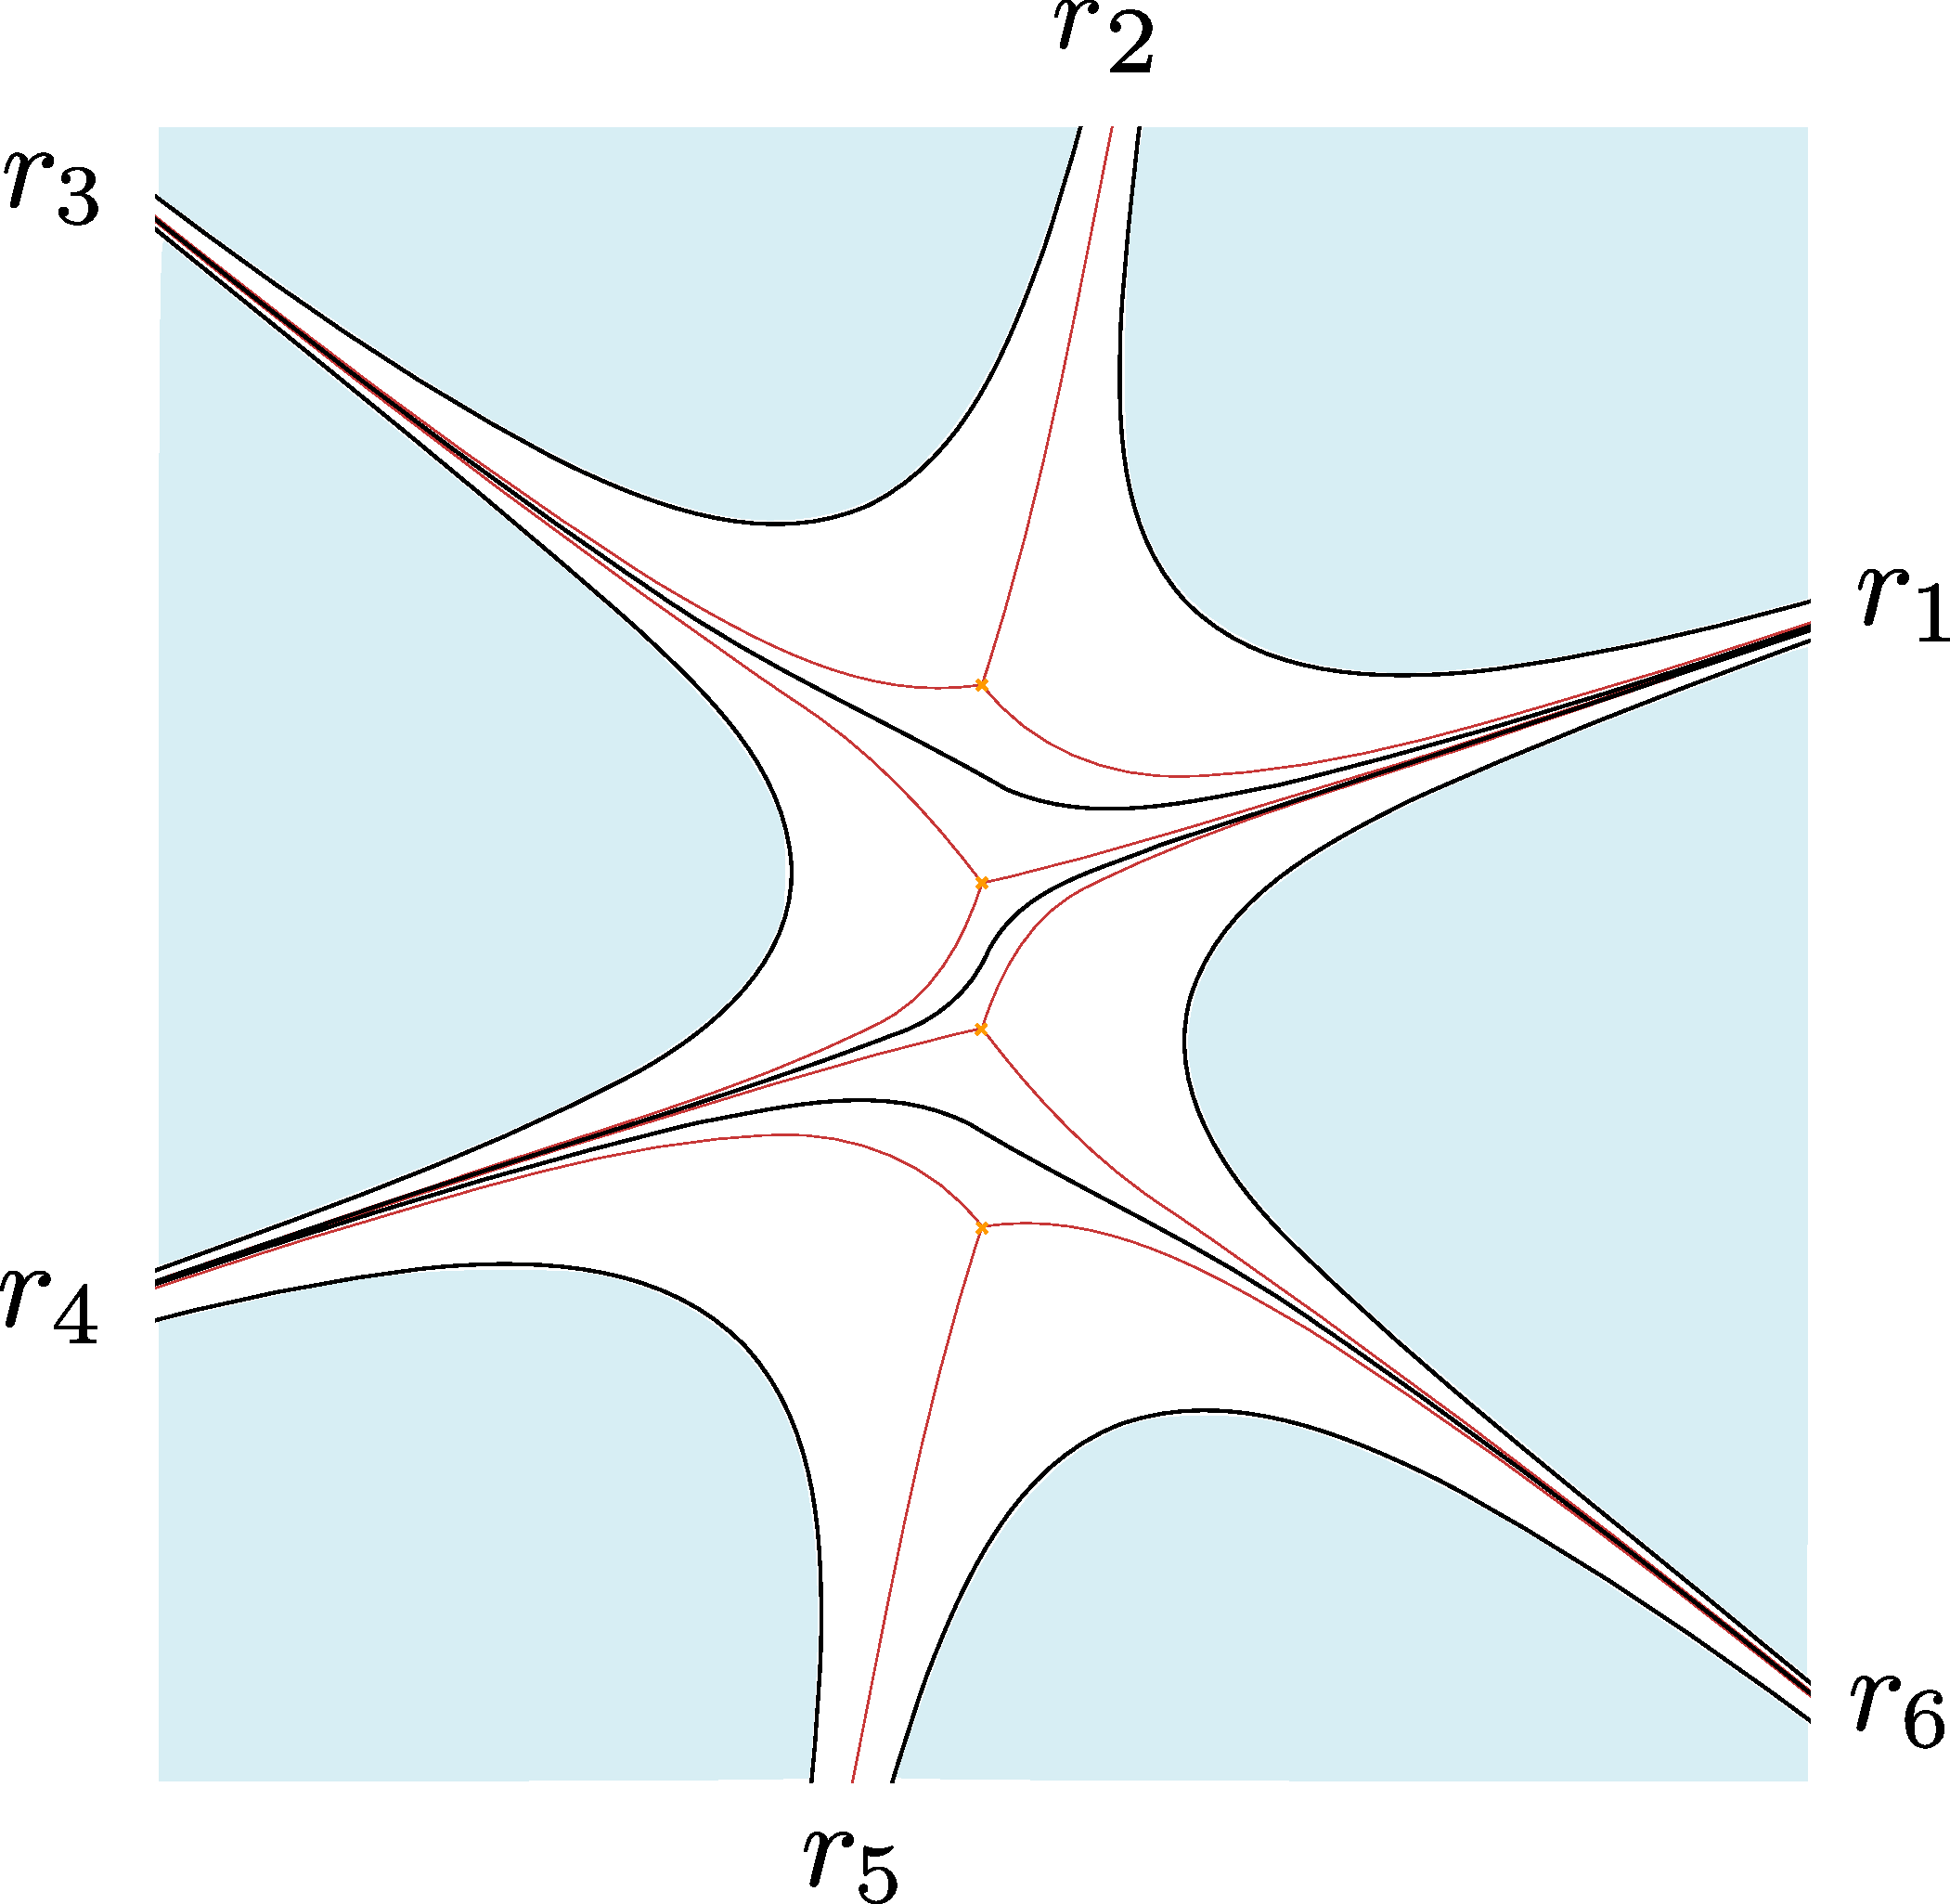
\includegraphics[width=2.75in]{figures/N4plot-crop.pdf}
\caption{$m=0$ 时 $N=4$ 的一个一般 WKB 三角剖分。}\label{fig:N4plot}
\end{minipage}
\hspace{0.4cm}
\begin{minipage}[b]{0.45\linewidth}
\centering 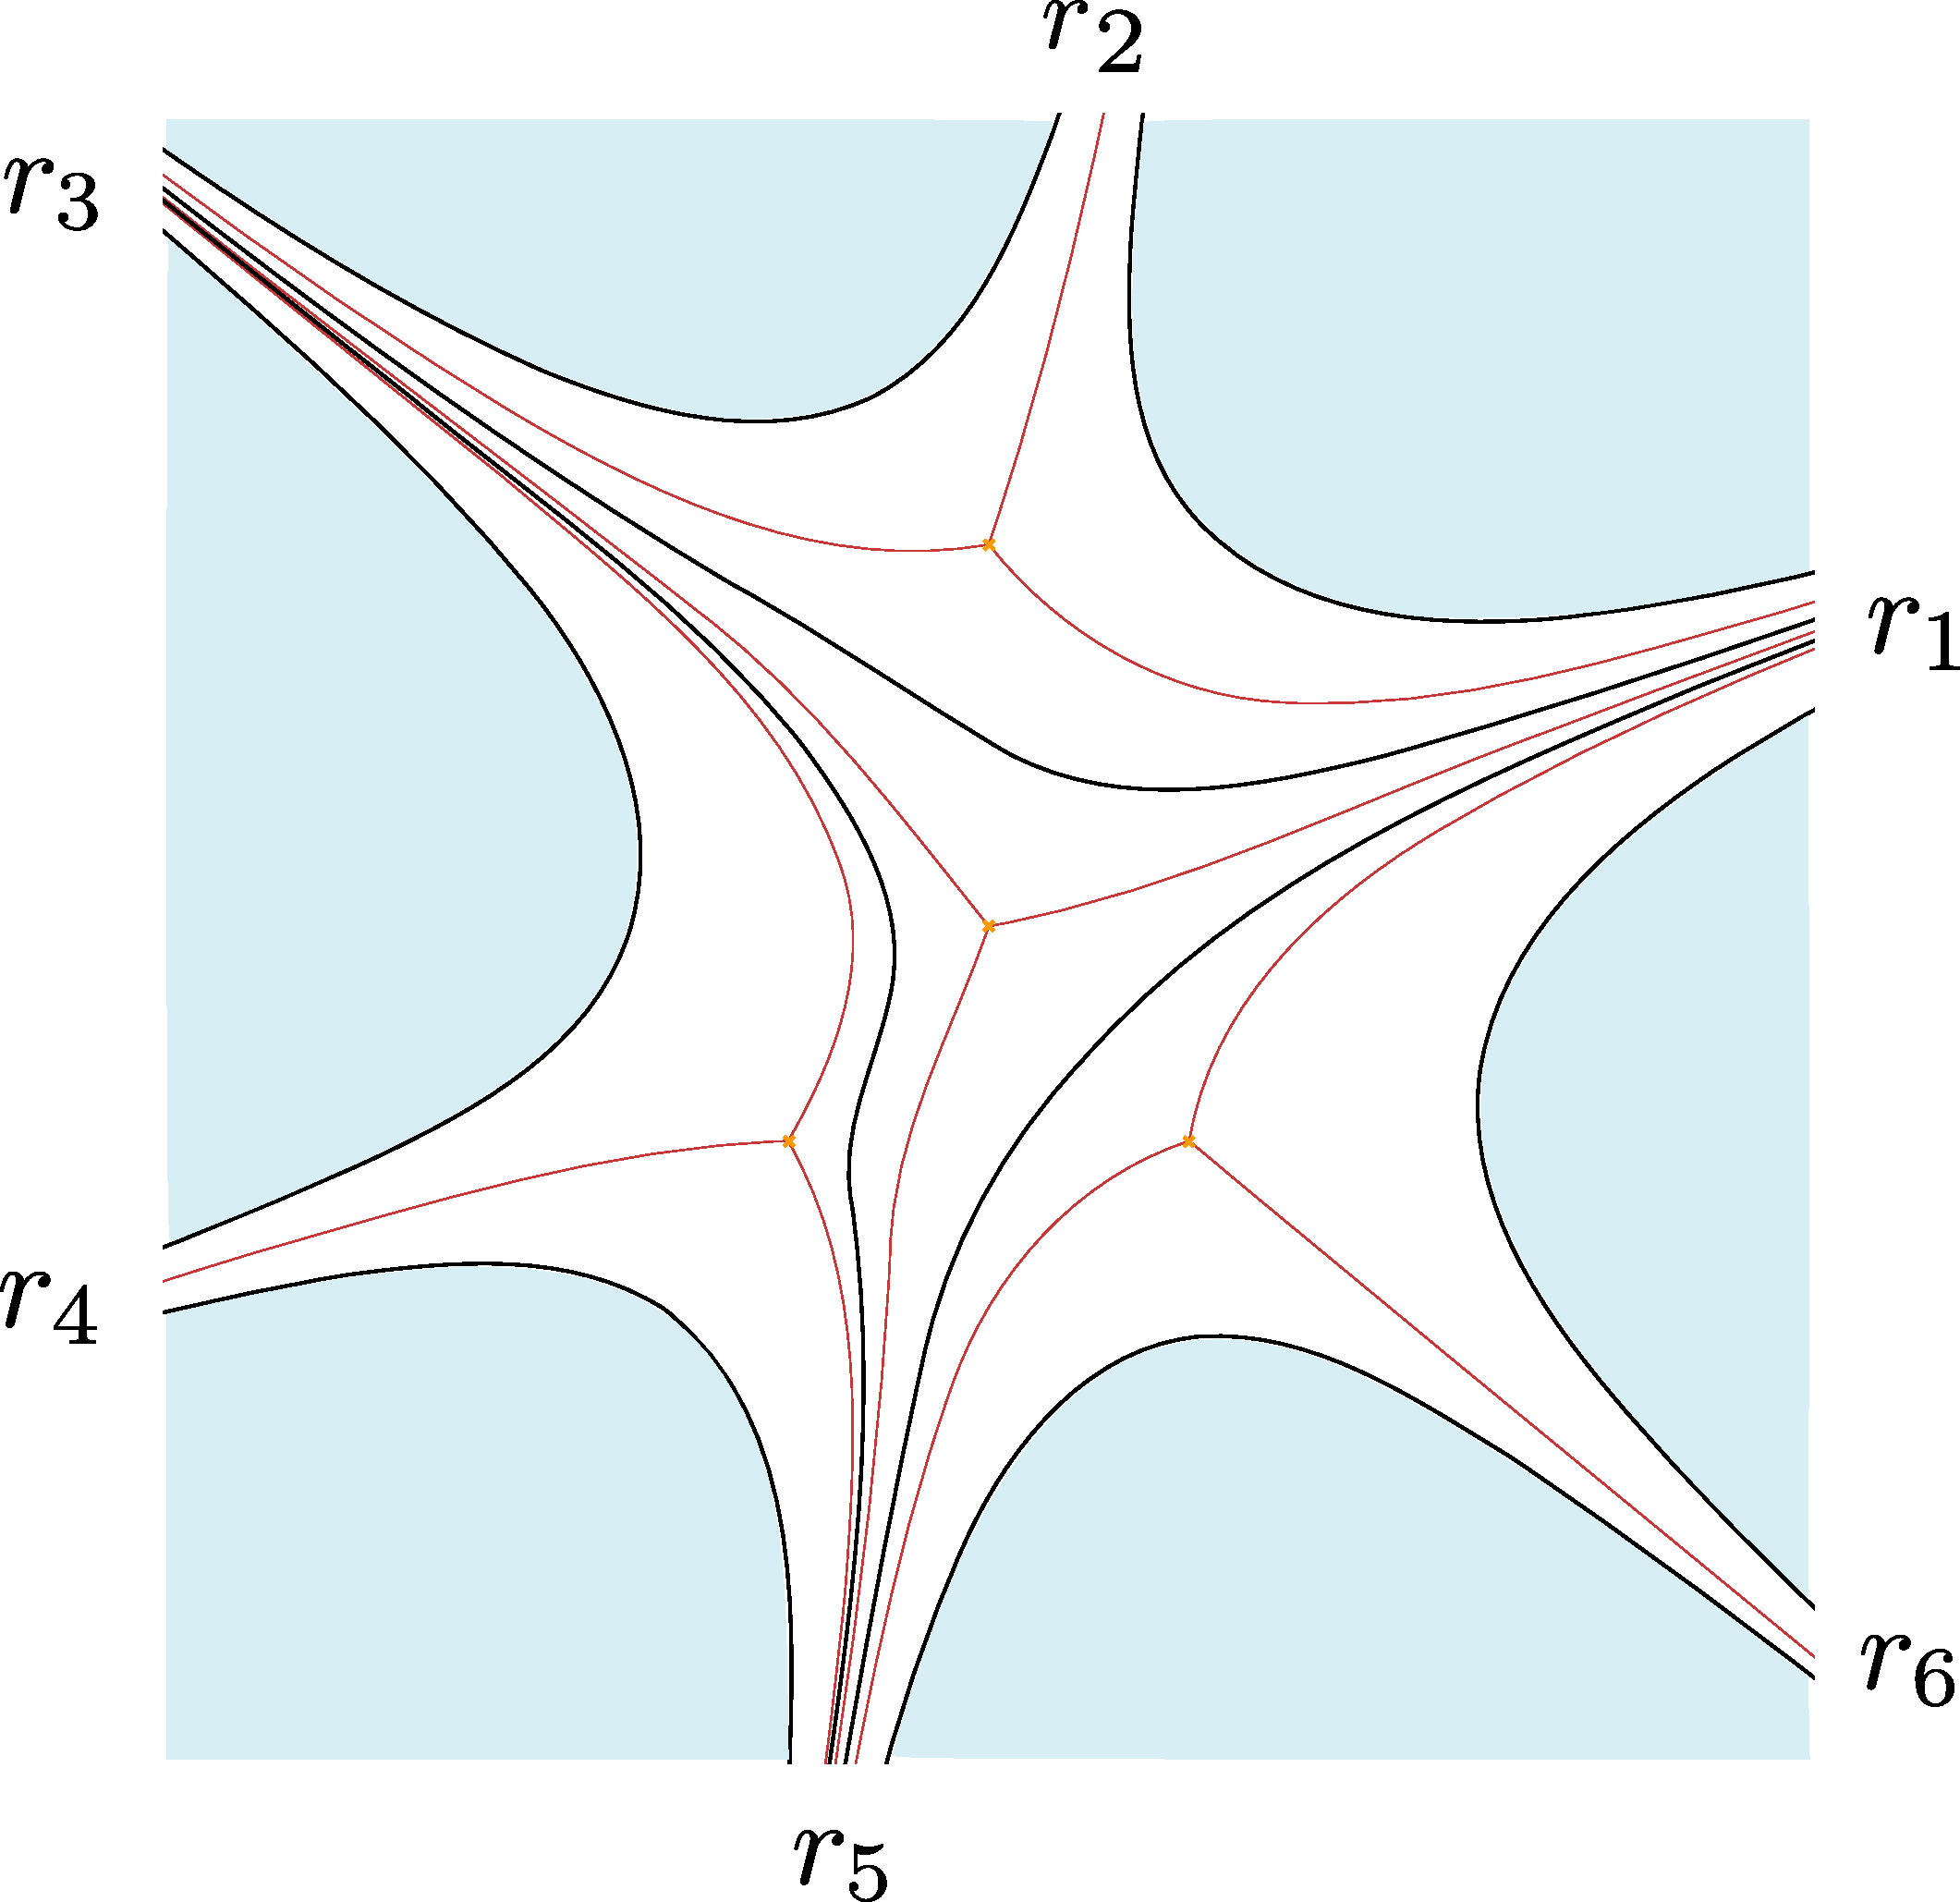
\includegraphics[width=2.75in]{figures/N4plotbis-crop.pdf}
\caption{$m$ 很大时 $N=4$ 的一个一般 WKB 三角剖分。}\label{fig:N4plotbis}
\end{minipage}
\end{figure}

此时 WKB 三角剖分给出的是六边形的三角剖分，如图 50、51 所示。所有可能的三角剖分都会在参数空间的某处出现。
% TODO 合稿改 \ref{fig:N4plot}、\ref{fig:N4plotbis}

下面来描述 BPS 谱。

\subsubsection*{$m=0$ 的情形}

先设 $m=0$ 是有用的。此时判别式退化为 $256 u(u - 4 \Lambda^4)^2$，于是 $\CB$ 中有两个奇点：

\begin{itemize}
\item 在 $u=0$ 处，$P(z)$ 的两个零点在 $z=0$ 处重合，而另外两个零点位于 $z = \pm 2 i \Lambda$。我们预期在这里看到一个 BPS 粒子变为无质量。
\item 在 $u=4 \Lambda^4$ 处，$P(z)$ 是一个完全平方，两对零点在 $z=\pm i \sqrt{2} \Lambda$ 处相撞。我们预期在这里看到两个不同的 BPS 粒子变为无质量。这两个粒子具有相同的规范荷，因为它们在 $\bar\Sigma$ 中对应的闭链同调；但它们的味荷不同。（确实，$\Sigma$ 上这两个对应闭链之差是一个绕 $z = \infty$ 的闭链。若取某个小的 $m \neq 0$，$\oint \lambda$ 就会给出那里单极点的留数 $m$。）
\end{itemize}

通过研究 $\CB$ 中的奇点结构，我们已经遇到了三个 BPS 粒子的效应。现在，让我们沿 $T_\WKB(\vartheta, u)$ 对 $\vartheta$ 的依赖关系，更有系统地考察 BPS 谱。先固定任意一个 $0 < u < 4 \Lambda^4$。此时四个转向点在 $z$-平面中共线，我们会遇到与相邻转向点之间的弦相对应的 BPS 态。把连接中间那两个转向点的 BPS 弦的荷记作 $\gamma_1$。另外两条 BPS 弦的荷记作 $\gamma_2$、$\gamma_3$，于是 $\gamma_2 + \gamma_3$ 是纯味荷（特别地，当 $m=0$ 时 $Z_{\gamma_2} + Z_{\gamma_3} = 0$）。我们取这样的约定：
\begin{equation}
\langle \gamma_3, \gamma_1 \rangle = \langle \gamma_1, \gamma_2 \rangle = 1,
\qquad \langle \gamma_2, \gamma_3 \rangle = 0.
\end{equation}
注意 $\CK_{\gamma_2}$ 与 $\CK_{\gamma_3}$ 对易，这个事实下面会反复用到。$\CB$ 中有一条边缘稳定墙，它穿过这两个奇点，并围住一个椭球状区域；该区域包含线段 $0<u \Lambda^{-4} <4$。\insfig{5.5in}{exa-evolution}{$m=0$ 时的 WKB 三角剖分。上条：在 $u=0$ 处，当 $\vartheta$ 从 $0$ 变到 $\pi$ 时，$T_\WKB$ 的演化很简单，共有三次 flip：在第一条蓝色点线处有一对彼此对易的 flip，在红线处有第三次 flip。下条：对超出边缘稳定墙的 $u$，$T_\WKB$ 以另一种方式演化，涉及六次 flip。在第二条与第四条点线处都发生两次 flip，对应两个荷相同的 BPS 粒子。注意 $T_\WKB(\vartheta)$ 与 $T_\WKB(\vartheta+\pi)$ 相同，只差 WKB 射线的一个重标号。} 现在，通过直接计算（手算或用计算机），就可以得到 $T_\WKB(\vartheta)$ 随 $\vartheta$ 的演化。在图 52 中我们画出了结果，其中取两个 $u$，一个在边缘稳定墙之内、一个在墙外。% TODO 合稿改 \ref{fig:exa-evolution}
在 $u=0$ 处，我们看到 $T_\WKB$ 中有三次 flip，对应三个 BPS 荷 $-\gamma_3$、$\gamma_2$、$\gamma_1$。当我们穿过边缘稳定墙时，中心荷 $Z_{\gamma_2}$、$Z_{-\gamma_3}$ 的相位会与 $Z_{\pm \gamma_1}$ 之一的相位对齐（取哪个符号，取决于我们穿过墙的哪一段）。在墙的另一侧，$T_\WKB$ 中的 flip 以不同的顺序发生，我们一共看到六个 BPS 超多重态。每一对转向点之间都有一条 BPS 弦。

于是，依照与上面 $N=3$ 情形类似的推理，我们必定有穿墙恒等式
\begin{equation} \label{eq:k-identity}
\CK_{\gamma_1} \CK_{\gamma_2} \CK_{-\gamma_3}
= \CK_{\gamma_2} \CK_{-\gamma_3} \CK_{\gamma_1+\gamma_2-\gamma_3} \CK_{\gamma_1+\gamma_2}\CK_{\gamma_1-\gamma_3}
\CK_{\gamma_1}.
\end{equation}
\eqref{eq:k-identity} 中因子的次序很容易理解，只需用到这样的事实：$Z_{\gamma_2} = Z_{-\gamma_3}$，并且当 $k_1, k_2$ 变动时，$Z_{k_1 \gamma_1 + k_2 \gamma_2}$ 的宗量的次序由 $k_1 / k_2$ 的次序决定。同样，人们可以显式检验 \eqref{eq:k-identity} 是一个真正的恒等式，但我们在下一段会给出一个更简单的证明。

\subsubsection*{$m \neq 0$ 的情形}

当 $m \neq 0$ 时，图像要稍复杂一些。对小的 $m$，荷为 $\gamma_2$ 与 $\gamma_3$ 的粒子在 $\CB$ 中略有不同的点处变为无质量。边缘稳定墙也分裂成若干条墙。于是穿墙公式 \eqref{eq:k-identity}「分解」为三个独立的五边形恒等式。一种可能的分解是
\begin{equation}
\begin{split}
\CK_{\gamma_1} \CK_{\gamma_2} \CK_{-\gamma_3}
&= \CK_{\gamma_2} \CK_{\gamma_1+\gamma_2} \CK_{\gamma_1} \CK_{-\gamma_3} \\
&= \CK_{\gamma_2} \CK_{\gamma_1+\gamma_2} \CK_{-\gamma_3} \CK_{\gamma_1-\gamma_3} \CK_{\gamma_1} \\
&= \CK_{\gamma_2} \CK_{-\gamma_3} \CK_{\gamma_1+\gamma_2-\gamma_3} \CK_{\gamma_1+\gamma_2}\CK_{\gamma_1-\gamma_3}
\CK_{\gamma_1},
\end{split}
\end{equation}
它对应三条彼此分离的边缘稳定墙：先是 $Z_{\gamma_1}$ 与 $Z_{\gamma_2}$ 对齐，然后是 $Z_{\gamma_1}$ 与 $Z_{-\gamma_3}$ 对齐，再是 $Z_{-\gamma_3}$ 与 $Z_{\gamma_1 + \gamma_2}$ 对齐。第二种可能是
\begin{equation}
\begin{split}
\CK_{\gamma_1} \CK_{\gamma_2} \CK_{-\gamma_3}
&= \CK_{-\gamma_3} \CK_{\gamma_1-\gamma_3} \CK_{\gamma_1} \CK_{\gamma_2} \\
&= \CK_{-\gamma_3} \CK_{\gamma_1-\gamma_3} \CK_{\gamma_2}\CK_{\gamma_1+\gamma_2} \CK_{\gamma_1} \\
&= \CK_{\gamma_2} \CK_{-\gamma_3} \CK_{\gamma_1+\gamma_2-\gamma_3} \CK_{\gamma_1+\gamma_2}\CK_{\gamma_1-\gamma_3}
\CK_{\gamma_1}.
\end{split}
\end{equation}
相应的 WKB 三角剖分序列如图 53 所示。% TODO 合稿改 \ref{fig:exa-evolution-mass}
\insfig{5.5in}{exa-evolution-mass}{上条：在 $u = 0$ 处，$T_\WKB(\vartheta, u)$ 随 $\vartheta$ 的演化很简单，只经历三次 flip。下条：当我们把 $u$ 变向 $\infty$ 时，会穿过三条墙。每穿过一条墙之后，我们画出 $T_\WKB(\vartheta, u)$ 随 $\vartheta$ 的新演化。在最后一条中，为节省篇幅，我们没有画出规范荷相同的成对 BPS 跳变之间的中间三角剖分。}

在图 54 中，我们画出 $\CB$ 中非常靠近 $Z_{\gamma_1} = 0$ 那个奇点处的墙的结构。墙的整体结构相当复杂，并且依赖于 $m$ 的相位。
% TODO 合稿改 \ref{fig:N4uplane-detail-a}

\insfig{3.3in}{N4uplane-detail-a}{$N=4$ 理论中的边缘稳定墙，画在满足 $Z_{\gamma_1}(u)=0$ 的点 $u$ 附近，取某种小 $m \neq 0$ 的选择。（对 $m$ 的其他相位，图中 $\gamma_2$ 与 $-\gamma_3$ 可能互换。）注意 $\hat\Gamma$ 有单值，因此需要橙色的割线。}

注意，可以沿一条更曲折的路径从小 $u$ 走到大 $u$：这条路径从 $Z_{\gamma_2} = 0$ 与 $Z_{\gamma_3} = 0$ 这两个奇点之间穿过。此时穿墙公式会以另一种方式排列，例如
\begin{equation}
\begin{split}
\CK_{\gamma_3} \CK_{\gamma_1} \CK_{\gamma_2}
&= \CK_{\gamma_1} \CK_{\gamma_1+\gamma_3} \CK_{\gamma_3} \CK_{\gamma_2} \\
&= \CK_{\gamma_1} \CK_{\gamma_2} \CK_{\gamma_1+\gamma_2+\gamma_3}\CK_{\gamma_1+\gamma_3} \CK_{\gamma_3} \\
&= \CK_{\gamma_2} \CK_{\gamma_1+\gamma_2}\CK_{\gamma_1} \CK_{\gamma_1+\gamma_2+\gamma_3}\CK_{\gamma_1+\gamma_3} \CK_{\gamma_3}.
\end{split}
\end{equation}
（记住 $\CK_{\gamma_3}$ 与 $\CK_{\gamma_2}$ 对易。）检验由「从内部区域经不同奇点对之间穿到外部区域」所生成的 BPS 谱，与电荷格绕各奇点自身的单值，二者是否自洽，是一件有趣味的练习。细节随 $m$ 的相位而变。

对 $m$ 作恰当的选择，可以把另一对奇点（比如 $Z_{\gamma_1} = 0$ 与 $Z_{\gamma_2} = 0$）拉到一起，从而在 $\CB$ 中产生一个标度区，看起来就像我们 $N=3$ 的例子。在这个极限下，我们看到一个中心区域，其中的 BPS 谱由下列粒子组成：在复合的 $N=3$ 奇点处变轻的粒子，荷为 $\gamma_2$、$\gamma_1+\gamma_2$、$\gamma_1$；以及在剩下的那个单奇点处变轻的粒子，荷为 $\gamma_3$。我们在图 55 中画出这一 $m$ 选择下 $\CB$ 的结构。$T_\WKB$ 的相应行为见图 56。
% TODO 合稿改 \ref{fig:N4uplane-c}；末句 TODO 改 \ref{fig:N4toN3plot}

\insfig{4.5in}{N4uplane-c}{$N=4$ 理论中的边缘稳定墙，取使奇点 $Z_{\gamma_1}=0$ 与 $Z_{\gamma_2}=0$ 相撞的那个特殊质量 $m$。在每个区域内部，我们按相位的次序（差一个整体的循环置换）列出该区域内谱中所有 BPS 超多重态的荷。在每条墙上，我们给出相应的穿墙公式。}

\insfig{3in}{N4toN3plot}{$N=4$ 理论的三角剖分 $T_\WKB$，其中 $m$ 与 $u$ 取成使三个转向点正在聚拢。在左侧，$N=3$ 例子的五边形结构在 $N=4$ 的三角剖分内部浮现出来。}

对一般的 $m$，在 $\abs{u}$ 足够大的地方有一个区域，那里的转向点大致排成一个正方形，有 6 个 BPS 态与它的边和对角线相关联。从这个行为我们得知：在一个一般的 $\CN=2$ 理论中，在库仑分支上四个转向点汇合的那种奇点附近，我们通常会找到六个轻的 BPS 粒子，它们实现为连接任意一对转向点的 BPS 弦。

\subsection{一般 $N$ 与结合面体}

最后，我们作一些对一切 $N$ 都适用的评述。这些理论中的有限 WKB 曲线已由 Shapere 与 Vafa 在 \cite{Shapere:1999xr} 中描述过，其目的正是研究 BPS 态。他们证明了：

\begin{itemize}
\item 一条有限 WKB 曲线出现的相位 $\vartheta$，由该 WKB 曲线在带穿刺点的平面 $\IC - \{ \CT_i \}$ 中的同伦类唯一决定。

\item 连接任意两个转向点的有限 WKB 曲线至多只有一条。因此 BPS 态只有\emph{有限}多个。

\item 任意两个转向点都可以用有限 WKB 曲线的一段段拼接起来连接（一般每一段的 $\vartheta$ 不同）。因此在库仑分支上任意一点 $u$ 处至少有 $N-1$ 个 BPS 态。

\item BPS 态的最小数目 $N-1$，例如在所有根 $P_N(z)$ 都为实数时达到。最大数目 $\half N (N-1)$，例如在 $P(z) = z^N-1$ 时达到。

\item 自 $N$ 个转向点中的每一个发出的三条分界 WKB 曲线，各自渐近到 $z=\infty$ 处的一条不同射线。

\item 不存在闭合的 WKB 曲线。
\end{itemize}

于是，一般的 WKB 曲线定义了以 $N+2$ 个顶点构成的凸多边形的一个三角剖分。（上面我们已对 $N = 1, 2, 3, 4$ 见过这样的例子。）这一观察开启了一条通往数学中一个丰富分支的联系。$(N+2)$-边形的三角剖分对偶于三价图（trivalent graph），也对应于带 $N+1$ 个终端点的有根二叉树，或等价地，对应于给 $N+1$ 个非结合变量 $x_1 \cdots x_{N+1}$ 的乘积加括号的方式。这类三角剖分的数目是卡塔兰数 $C_N = \frac{1}{N+1} \binom{2N}{N}$。此外，$(N+2)$-边形的三角剖分可以看作一个单纯复形 $\CK_{N+1}$ 的顶点，其中 1-单纯形对应 flip。这个复形就是第 $N$ 个「结合面体」（associahedron），即 Stasheff 多面体的 1-骨架 \cite{MR0158400}。（近期的讨论可参见 \cite{Lee,MR1841954}。）$\CK_3$ 是一条线段，$\CK_4$ 是一个五边形。\cite{MR0158400} 的一个基本引理是：结合面体的面是低维结合面体的乘积。于是特别地，2-胞腔是五边形（对应五边形关系）与四边形（对应「不相交的边上的 flip 彼此对易」这一关系）。另一方面，结合面体本身是单连通的，因此它的二维骨架也是单连通的。\footnote{这一陈述也与范畴论中的 MacLane 相干性定理密切相关 \cite{MR0330253}。} 在我们的语境中，这意味着这些例子里出现的所有穿墙公式都是五边形关系的推论。我们在上面的 $N=3,4$ 例子中已经看到了这一事实。

结合面体在这类例子中的出现，引出了一个问题：$A_\infty$ 代数的理论在这里是否也有有趣的角色可扮演？另一个自然的问题是：若只给出多项式 $P(z)$，是否存在一个计算 BPS 态谱的简单算法？第 11 节% TODO 合稿改 \ref{sec:UniversalStokesMatrix}
中对谱生成元的计算，对第二个问题给出了肯定的回答。
